\documentclass[mathNotesPreamble]{subfiles}
\begin{document}
%\relscale{1.4} %TODO
\section{13.3: Dot Products}
  \begin{defn*}[Dot Product]
    Given two nonzero vectors $\bfu$ and $\bfv$ in two or three dimensions, their \textbf{dot product} is
      \[\bfu\cdot\bfv=\abs{\bfu}\abs{\bfv}\cos\theta,\]
    where $\theta$ is the angle between $\bfu$ and $\bfv$ with $0\leq \theta\leq \pi$. If $\bfu=\bfO$ or $\bfv=\bfO$, then $\bfu\cdot\bfv=0$, and $\theta$ is undefined.
  \end{defn*}
  %TODO Pick the two definitions of the dot product

  \begin{center}
    \begin{tikzpicture}
      \node[matrix, column sep=2.5mm]
      {
        \coordinate (O) at (0,0);
        \coordinate (A) at (-1.25,0);
        \coordinate (B) at (1.5,0);
        \draw[->, ClemsonOrange, line width=1.25pt] (O) -- (A)
          node[above, pos=0.5, black] {$\bfu$};
        \draw[->, ClemsonPurple, line width=1pt] (O) -- (B)
          node[above, pos=0.5, black] {$\bfv$};&
        %
        \coordinate (O) at (0-0.5,0);
        \coordinate (A) at (-1-0.5,1);
        \coordinate (B) at (2-0.5,0);
        \draw[->, ClemsonOrange, line width=1pt] (O) -- (A)
          node[above, pos=0.5, black, xshift=5pt, yshift=5pt] {$\bfu$};
        \draw[->, ClemsonPurple, line width=1pt] (O) -- (B)
          node[below, pos=0.5, black] {$\bfv$};
        \tkzFillAngle[fill= ClemsonOrange!90,size=0.45cm, opacity=0.8](B,O,A);
        \tkzLabelAngle[pos = 0.25,font=\normalsize](B,O,A){\color{black}$\theta$};&
        %
        \coordinate (O) at (0-0.75,0);
        \coordinate (A) at (0-0.75,2);
        \coordinate (B) at (2-0.75,0);
        \draw($(O)!0.125!(A)$)-|($(O)!0.125!(B)$);
        \draw[->, ClemsonOrange, line width=1pt] (O) -- (A)
          node[black, pos=0.5, xshift=-10pt] {$\bfu$};
        \draw[->, ClemsonPurple, line width=1pt] (O) -- (B)
          node[below, pos=0.5, black] {$\bfv$};&
        %
        \coordinate (O) at (0-1,0);
        \coordinate (A) at (1.414-1,1.414);
        \coordinate (B) at (2-1,0);
        \draw[->, ClemsonOrange, line width=1pt] (O) -- (A)
          node[above, pos=0.5, black, xshift=-5pt] {$\bfu$};
        \draw[->, ClemsonPurple, line width=1pt] (O) -- (B)
          node[below, pos=0.5, black] {$\bfv$};
        \tkzFillAngle[fill= ClemsonOrange!90,size=0.75cm, opacity=0.8](B,O,A);
        \tkzLabelAngle[pos = 0.55,font=\normalsize](B,O,A){\color{black}$\theta$};&
        %
        \coordinate (O) at (0-1.5,0);
        \coordinate (A) at (3-1.5,0.025);
        \coordinate (B) at (2-1.5,0);
        \draw[->, ClemsonOrange, line width=1.25pt] (O) |- (A)
          node[above, pos=0.85, black] {$\bfu$};
        \draw[->, ClemsonPurple, line width=1pt] (O) -- (B)
          node[below, pos=0.5, black] {$\bfv$};\\
        %
        \node[draw=black, rounded corners, font=\normalsize]
          {$\theta=\pi,\ \bfu\cdot\bfv=-\abs{\bfu}\abs{\bfv}$};&
        \node[draw=black, rounded corners, font=\normalsize]
          {$\bfu\cdot\bfv=\abs{\bfu}\abs{\bfv}\cos\theta<0$};&
        \node[draw=black, rounded corners, font=\normalsize]
          {$\theta=\frac{\pi}{2},\ \bfu\cdot\bfv=0$};&
        \node[draw=black, rounded corners, font=\normalsize]
          {$\bfu\cdot\bfv=\abs{\bfu}\abs{\bfv}\cos\theta>0$};&
        \node[draw=black, rounded corners, font=\normalsize]
          {$\theta=0,\ \bfu\cdot\bfv=\abs{\bfu}\abs{\bfv}$};\\
      };
    \end{tikzpicture}
  \end{center}
  \vspace*{\stretch{1}}

  \noindent
  A physical example of the dot product is the amount of work done when a force is applied at an angle $\theta$ as shown in figure 13.43:
  \begin{center}
    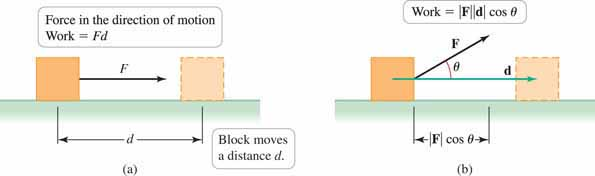
\includegraphics[width=0.75\linewidth]{images/briggs_13_03/fig13_43}
    
    \textit{Note}: The result of the dot product is a scalar!
    %TODO LC The result of the dot product is (a scalar, another vector,...)
    %TODO Think of "multiply the length they have in common"
  \end{center}
  \vspace*{\stretch{0}}
  \pagebreak
  
  \begin{defn*}[Orthogonal Vectors]
    Two vectors $\bfu$ and $\bfv$ are \textbf{orthogonal} if and only if $\bfu\cdot\bfv=0$. The zero vector is orthogonal to all vectors. In two or three dimensions, two nonzero orthogonal vectors are perpendicular to each other.
  \end{defn*}
  \begin{itemize}
    \item $\bfu$ and $\bfv$ are parallel ($\theta=0$ or $\theta=\pi$) if and only if $\bfu\cdot\bfv=\pm\abs{\bfu}\abs{\bfv}$.
    \item $\bfu$ and $\bfv$ are perpendicular ($\theta=\frac{\pi}{2}$) if and only if $\bfu\cdot\bfv=0$.
  \end{itemize}
  %TODO examples of computing the dot product
  
  \noindent
  \fbox{\parbox{0.9875\linewidth}{
    \textbf{Theorem 31.1: Dot Product}
    
    Given two vectors $\bfu=\bracket{u_1,u_2,u_3}$ and $\bfv=\bracket{v_1,v_2,v_3}$, 
      \[\bfu\cdot\bfv=u_1v_1+u_2v_2+u_3v_3.\]
  }}
  %TODO Outline of proof
  %TODO examples finding the angle between vectors
  \pagebreak
  
  \textbf{Properties of Dot Products}
  
  \noindent
  \fbox{\parbox{0.9875\linewidth}{
    \textbf{Theorem 13.2: Properties of the Dot Product}
    
    Suppose $\bfu, \bfv$ and $\bfw$ are vectors and let $c$ be a scalar.
    \begin{center}
      \begin{minipage}{0.7\linewidth}
        \TabPositions{0.6\linewidth}
        \begin{enumerate}
          \item 
            $\bfu\cdot \bfv =\bfv\cdot\bfu$ 
            \tab \textcolor{blue}{Commutative property}
          \item 
            $c\parens{\bfu\cdot\bfv}=\parens{c\bfu}\cdot \bfv=\bfu\cdot\parens{c\bfv}$
            \tab \textcolor{blue}{Associative property}
          \item 
            $\bfu\cdot\parens{\bfv+\bfw}=\bfu\cdot\bfv+\bfu\cdot\bfw$
            \tab \textcolor{blue}{Distributive property}
        \end{enumerate}
      \end{minipage}
    \end{center}
  }}
  %TODO LC pick out properties of dot product
  \pagebreak

  \textbf{Orthogonal Projections}

  \noindent
  Given vectors $\bfu$ and $\bfv$, the projection of $\bfu$ onto $\bfv$ produces a vector parallel to $\bfv$ using the ``shadow'' of $\bfu$ cast onto $\bfv$.
  \begin{center}
    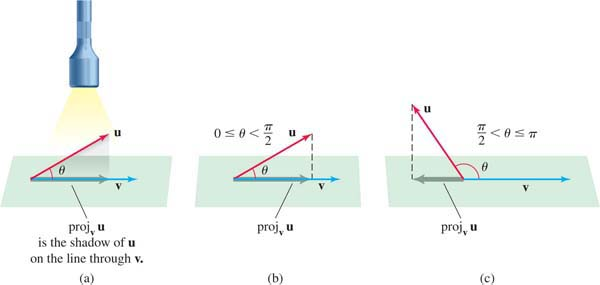
\includegraphics[width=0.9\linewidth]{images/briggs_13_03/fig13_47}
  \end{center}
%  \vspace*{\stretch{1}}
  %TODO "derive" projection
  %TODO LC How does |v|*|v| = v\cdot v?
  \begin{defn*}[(Orthogonal) Projection of $\bfu$ onto $\bfv$]
    The \textbf{orthogonal projection of $\bfu$ onto $\bfv$}, denoted $\proj_\bfv \bfu$, where $\bfv\neq\bfO$, is
      \[\proj_\bfv \bfu =\underbrace{\abs{\bfu}\cos\theta}_{\textnormal{\textcolor{blue}{length}}}\underbrace{\parens{\frac{\bfv}{\abs{\bfv}}}}_{\textnormal{\textcolor{blue}{direction}}}.\]
    The orthogonal projection may also be computed with the formulas
      \[\proj_\bfv \bfu=\operatorname{scal}_\bfv \bfu\parens{\frac{\bfv}{\abs{\bfv}}}=\parens{\frac{\bfu\cdot\bfv}{\bfv\cdot\bfv}}\bfv,\]
    where the \textbf{scalar component of $\bfu$ in the direction of $\bfv$} is
      \[\operatorname{scal}_\bfv \bfu=\abs{\bfu}\cos\theta=\frac{\bfu\cdot\bfv}{\abs{\bfv}}.\]
  \end{defn*}
  \pagebreak
  %TODO examples computing proj_v u and scal_v u
  \textbf{Applications of Dot Products}

  \begin{defn*}[Work]
    Let a constant force $\mathbf{F}$ be applied to an object, producing a displacement $\mathbf{d}$. If the angle between $\mathbf{F}$ and $\mathbf{d}$ is $\theta$, then the \textbf{work} done by the force is
      \[W=\abs{\mathbf{F}}\abs{\mathbf{d}}\cos\theta=\mathbf{F}\cdot \mathbf{d}\]
  \end{defn*}
  %TODO work example
  \begin{ex*}
    
  \end{ex*}
  
  \noindent
  \underline{Parallel and Normal Forces:}
  
  \noindent
  \begin{minipage}[t]{0.65\linewidth}
    \begin{ex*}
      %TODO parallel and normal forces example
    \end{ex*}
  \end{minipage}%
  {\begin{minipage}[t]{0.35\linewidth}\mbox{}
    \begin{flushright}
      \def\angle{35}
      \def\boxWidth{0.7}
      \def\scaleFact{1.6}
      \begin{tikzpicture}[
        M/.style={rectangle,draw,fill=ClemsonOrange!60,minimum size=2*\boxWidth cm,thin},
        plane/.style={draw=black,fill=ClemsonPurple!20},
        ]

        \draw[plane] (0,-1) coordinate (base)
                       -- coordinate[pos=0.5] (mid) ++(\angle:6) coordinate (top)
                       |- (base) coordinate[pos=0.5] (corner) -- cycle;
        \tkzFillAngle[fill= ClemsonOrange!90,size=0.85cm, opacity=0.8](corner,base,top);
        \tkzLabelAngle[pos = 0.65,font=\normalsize, yshift=0.5pt](corner,base,top){\color{black}$\theta$};
        \path (mid) node[M,rotate=\angle,yshift=\boxWidth cm] (M) {};
        \draw[->, line width=1pt, red] 
          ($(mid)+({-sin(\angle)*\boxWidth cm}, {cos(\angle)*\boxWidth cm})$) 
            -- ++(-90:5/\scaleFact) coordinate (gravity) 
          node[below, black, font=\normalsize, align=center] 
            {$\mathbf{F}$= gravitational force \\ (weight)};
        \draw[->, line width=1pt, blue] 
          ($(mid)+({-sin(\angle)*\boxWidth cm}, {cos(\angle)*\boxWidth cm})$) 
            -- ++(35-90:4/\scaleFact) coordinate (normal)
          node[right, pos=0.5, black, font=\normalsize, align=right] 
            {Normal\\ component\\ of $\mathbf{F}$};
        \draw[->, line width=1pt, blue] 
          ($(mid)+({-sin(\angle)*\boxWidth cm}, {cos(\angle)*\boxWidth cm})$) 
            -- ++(35-180:3/\scaleFact) coordinate (parallel)
          node[above left, anchor=east, black, font=\normalsize, align=left,
            yshift=10pt, pin={[pin edge={->, shorten >=9pt}]0:{}}] 
            {Parallel\\ component\\ of $\mathbf{F}$};
        \draw[dashed, blue] (normal) -- (gravity) -- (parallel);
      \end{tikzpicture}
    \end{flushright}
  \end{minipage}}
\pagebreak


\end{document}
